% -----
% COMP2550/COMP3130 Warmup Project Report
% CHRISTOPHER CLAOUE-LONG
% -----

% DELIVERABLES:
%You need to submit your source code (in a tarball) and a two page technical report (as a PDF). Your report should include a description of your features, some example results (pictures), a numerical analysis of your algorithm, and answers to the following questions:
%� What is the performance of your algorithm on the training set compared to the test set? Is this result expected?
%� Why is it important to evaluate pixelwise accuracy instead of accuracy on the superpixels? � What do you think is more important, the features or the machine learning classifier?
%The software and two page report are due at 11:59pm on 22 March, 2012.
% -
% - DOCUMENT GEOMETRY SETUP
\documentclass[11pt,a4paper]{article}
\usepackage{geometry}
\geometry{top=18mm,bottom=18mm,left=20mm,right=20mm}
\usepackage{lastpage}
\makeatletter \renewcommand{\@oddfoot}{\hfil Page \thepage\ of \pageref{LastPage} \hfil} \makeatother
% -
% - SECTION FORMATTING
\renewcommand \thepart{\Roman{part}}
\renewcommand \thesection{\arabic{section}}
\renewcommand \thesubsection{\arabic{section}.\arabic{subsection}}
\renewcommand \thesubsubsection{\arabic{section}.\arabic{subsection}.\arabic{subsubsection}}
% -
% - FONT
\usepackage{amsmath, amsthm, amssymb,graphicx,epstopdf}
\DeclareGraphicsRule{.tif}{png}{.png}{`convert #1 `dirname #1`/`basename #1 .tif`.png}
\usepackage[sc]{mathpazo}
\linespread{1.05}
\usepackage[T1]{fontenc}
\usepackage[bitstream-charter]{mathdesign}
% -
% - MISC. PACKAGES
\usepackage{color}
\usepackage[usenames,dvipsnames,svgnames,table]{xcolor}\usepackage{tikz} \usepackage{qtree, tikz-qtree, lineno}
\renewcommand\linenumberfont{\normalfont\sffamily}
\usepackage{datetime, multicol, verbatim, ulem, alltt, multirow, hyperref}
\hypersetup{
colorlinks,
citecolor=black,		% - Citation colour
filecolor=black,		% - File colour
linkcolor=black,		% - Link colour
urlcolor=black		% - URL colour
}
\urlstyle{same}
% -
% -
% - MISC. SYMBOLS AND COMMANDS
% - Thick horizontal blue line
\newcommand{\Hrule}{\textcolor{blue}{\rule{\linewidth}{0.5mm}}}
\newcommand{\HUGEBOLD}[1]{\textbf{\Huge{#1}}}
% -----
\begin{document}
% -----
% - Title
{\center
\textbf{\Huge COMP2550/COMP3130 ANU\\Warmup Project Report}\\
\textbf{\\\large Christopher Claou\'e-Long 
(\href{mailto:u5183532@anu.edu.au}{\textit{\underline{\smash{u5183532@anu.edu.au}}}})\\
Jimmy Lin 
(\href{mailto:u5223173@anu.edu.au}{\textit{\underline{\smash{u5223173@anu.edu.au}}}})\\}
}
% -
% -
\begin{multicols*}{2}
\section{Introduction and Overview}
The field of computer vision is often thought of as a diverse topic, with many different projects achieving different goals. In reality, there are three major paths to which each project can be linked.  The first two -- scene categorisation and object detection -- aim to provide a partial summary of a scene using tags or bounding boxes around discrete objects, however do not deliver an accurate object outline nor consider the image as a whole like what happens in real life human vision.

The task for this warmup project was to perform research along the third major path: annotating an entire image at the pixel level to describe the entire scene.  This would be done by considering a unified cluster of pixels (a superpixel) and extracting a set of useful 's open source Darwin framework for machine learning on the MSRC dataset.  The desired outcome was a feature vector that allowed the machine learning classifier to differentiate superpixels in images with at least 50\% accuracy, and to identify whether a good classifier or good set of features is more important to achieve accurate computer vision.

\section{Method}
It is hypothesised that a set of good features will be more important to correct image labelling than achieving an efficient and complex classifier, therefore the features must reflect on how humans view images.

The human species has developed a striking ability to differentiate objects based on their colour alone.  To this extent, the first features considered were based on this to begin separating between superpixels of obvious colour difference. Calculating the average value of discrete red, green and blue values and their standard deviation across the superpixel appears to be a valid, if na\"ive method of approximating this. Including the average difference and absolute difference between the discrete primary colour values at each pixel position and those immediately neighbouring them is hypothesised to also increase accuracy..

Although colour is one of humans' primary resources when differentiating objects, it alone is insufficient to work out what an object is in an image.  Position is another important feature to include, especially when the need arises to differentiate between sky and water or trees and grass for example.  To approximate this aspect of human vision, the feature vector also contains the average position of the superpixel -- its centre -- and a standard deviation of the x and y coordinates it contains.
 
Real life vision does not only take into consideration the immediate features of a discrete object.  Whenever the eye looks at a point of interest, it also captures data from around it to work out the shape and outline of objects of import.  The average colour of the neighbouring superpixels is therefore also factored in as this is hypothesized to increase the probability of an accurate judgement about the superpixel label based on what it is surrounded by.

The classifier relies on a decision tree with a default maximum depth of 8 and a threshold cutoff of 1000.  Increasing these values may lead to an overall improvement in accuracy as well.%  To check this accuracy, Pixelwise labelling will be used to ensure that superpixels do not `leak' across multiple objects.
\section{Results}

\begin{tabular}{|p{100pt}|p{50pt}|p{50pt}|}\hline
Description & Accuracy on test data  & Accuracy on training data\\\hline
Only colour features taken into consideration & 50.42\% & 53.77\%\\\hline
Only colour features and position taken into consideration & 51.24\% & 57.59\%\\\hline
Fully featured algorithm& 52.33\% & 57.99\%\\\hline
As above (threshold cutoff of 2000) & 52.24\% & 57.93\%\\\hline
As above (threshold cutoff of 2000 and maximum depth of 16) & 53.14\% & 70.46\% \\\hline
\end{tabular}
\end{multicols*}\newpage
\begin{multicols*}{2}

% Grass
\noindent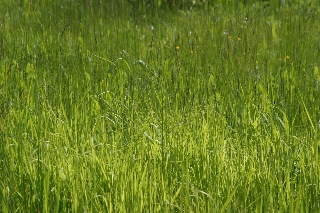
\includegraphics[scale=0.0045]{images/act1_3_s.jpg}\ \ \ \ \ \ \ \ \ \ \ \ \ 

\includegraphics[scale=0.33]{images/perc1_3_s.png}\\

% Trees
\ \ \ \noindent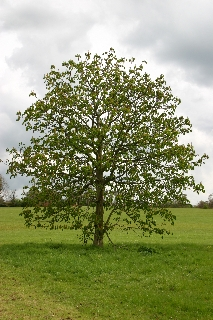
\includegraphics[scale=0.005]{images/act2_18_s.jpg}\ \ \ 
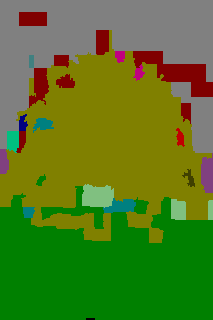
\includegraphics[scale=0.35]{images/perc2_18_s}\\

% Books
\noindent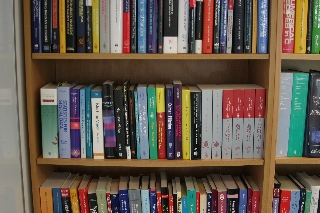
\includegraphics[scale=0.0048]{images/act13_7_s.jpg}\ \ \ \ \ \ \ \ \ \ \ \ \  

\includegraphics[scale=0.34]{images/perc13_7_s}\\

% House on grass
\noindent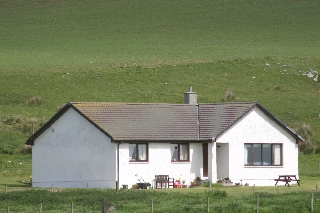
\includegraphics[scale=0.0048]{images/act3_12_s.jpg}\ \ \ \ \ \ \ \ \ \ \ \ \ 
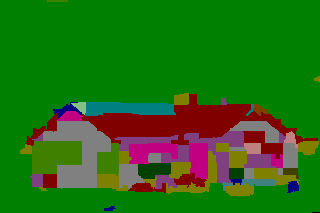
\includegraphics[scale=0.34]{images/perc3_12_s}\\
\textit{The classifier can differentiate accurately between values of similar colour and different contrast, but labels a cloudy sky mostly grey because to it, the features of the sky look like those of a building (right colour, right position, neighbours of similar colour).}\\
\textit{When given a complex scene with many objects, the classifier fails to achieve high accuracy.  It manages to differentiate obvious outlines, but incorrectly labels superpixels that are not immediately obvious from their colour and position features.}

\section{Discussion}
Pixelwise label checking was required to ensure the accuracy of the features and classifier, since as shown on the images above a superpixel may overlap onto multiple different objects -- making it impossible to check whether the superpixel was labelled correctly.  Pixelwise checking avoids this problem since it has no possible overlap, there is no smaller unit.  This ensures that the overall accuracy of the machine learning algorithm is measured correctly.

The resulting images and average accuracy results of the algorithm show that when faced with a simple picture with objects of vastly different colour and contrast, the classifier has enough knowledge from the features to differentiate between them.  However, as soon as it is given a picture with ambiguous colour and contrast or a complex set of multicoloured objects, accuracy reduces dramatically.  The problem therefore resides in the feature set's inability to differentiate the various peak colours in the superpixels; this is most notable in images where objects are similar in colour or where there is a large amount of different objects since the object labels `leak' into the background considerably.

Increasing the cutoff threshold of the decision tree had a slight negative effect on the accuracy of the classifier without the addition of a deeper tree cutoff.  However, the accuracy gained on the test set was very small in comparison to the accuracy on the training data, which improved considerably -- this suggests that while it is normal to achieve higher accuracy on the data the algorithm trained on, the implemented features are overfitting to the training dataset.

The accuracy also confirmed the hypothesis that achieving a good set of features is more important than devising a clever and more complex classifier -- even with a simple decision tree classifier, the results were only as accurate as the features it was given allowed; increasing the decision complexity had very little effect. The implementation of a set of good, well thought out features that allow the classifier to accurately differentiate data is therefore essential to a computer's whole-image understanding.

Possible improvements to the feature set in order to achieve a better labelling of superpixels therefore need to discriminate especially between texture and peak colour content of superpixels -- to this end taking into account the hue, peak colour histogram values, improved neighbour algorithms, and applying a gaussian/laplacian filter to statistically analyse the texture of the superpixel would be a good avenue for further research. 
\section{Project Reference}
K. Park and S. Gould. On Learning Higher-Order Consistency Potentials for Multi-class Pixel Labeling, \textit{Proceedings of the European Conference on Computer Vision (ECCV)}, 2012.\\
S. Gould. DARWIN: A Framework for Machine Learning and Computer Vision Research and Development, \textit{JMLR}, 2012.
\end{multicols*}

\end{document}
% -----
% END OF LINE
% -----
